\documentclass[aspectratio=169]{beamer}

\usetheme{Madrid}
\usepackage{booktabs}
\usepackage{graphicx}
\usepackage{listings}
\usepackage{xcolor}
\setbeamertemplate{navigation symbols}{}
\setbeamertemplate{caption}{\raggedright\insertcaption\par}

% compact JSON-ish listing style for the card drafts
\definecolor{kf}{HTML}{1f6feb}
\definecolor{cm}{HTML}{6a737d}
\lstdefinestyle{json}{
  basicstyle=\ttfamily\scriptsize,
  breaklines=true, columns=fullflexible,
  showstringspaces=false,
  keywordstyle=\color{kf}, commentstyle=\color{cm}\itshape,
  morecomment=[l]{//}, morekeywords={},
  frame=none, aboveskip=2pt, belowskip=2pt
}

\title[Model \& Dataset cards for LULC]{A schema for the LULC model \& dataset zoo}
\subtitle{Model cards, dataset cards, and the catalogue that ties them together}
\author[Salil Gujar]{Salil Gujar \\ \footnotesize M.Tech CSE \quad Entry No.\ 2025MCS2106}
\date{June 2026}

\begin{document}

\frame{\titlepage}

% ------------------------------------------------------------------
\begin{frame}{Where we are, and the direction}
\begin{columns}[T]
\begin{column}{0.5\textwidth}
\textbf{Done so far}
\begin{itemize}\small
  \item A 4-class base map (greenery / water / built-up / barren) from Alpha Earth, at 10\,m.
  \item A \textbf{living hierarchy}: split / add a class at any level, retrain on the fly,
  and the map updates, with metrics.
\end{itemize}
\end{column}
\begin{column}{0.5\textwidth}
\textbf{The direction (what was advised)}
\begin{itemize}\small
  \item build a \textbf{model zoo + dataset catalogue} with design.
  \item Each model tagged with \emph{where it's valid}, what it emits, what it trained on,
  and how classes were annotated. We call these ``model cards''.
  \item Let users browse, pick one for their area, and keep refining.
\end{itemize}
\end{column}
\end{columns}
\vspace{0.6em}
\centering
\end{frame}

% ------------------------------------------------------------------
\begin{frame}{The structure: two record types (+ a spine)}
What the schema defines is the \emph{shape} of each record, not any one model:
\begin{itemize}
  \item \textbf{Dataset Card}: a labeled \emph{source} (polygons, an EE asset, or a pixel
  table) with a description, spatial/temporal extent, provenance/evidence, and quality.
  \item \textbf{Model Card}: a \emph{classifier} at one node, holding the classes it emits,
  the datasets it trained on, where it's valid, its metrics, and how it deploys.
  \item \textbf{Canonical taxonomy}: the 4 base classes the cards hang off.
  \item \textbf{Catalogue}: a flat JSON registry of cards plus an index, queried to pick a
  model for an area.
\end{itemize}
\vspace{0.5em}

\end{frame}

% ------------------------------------------------------------------
\begin{frame}{The class tree the cards hang off}
\centering
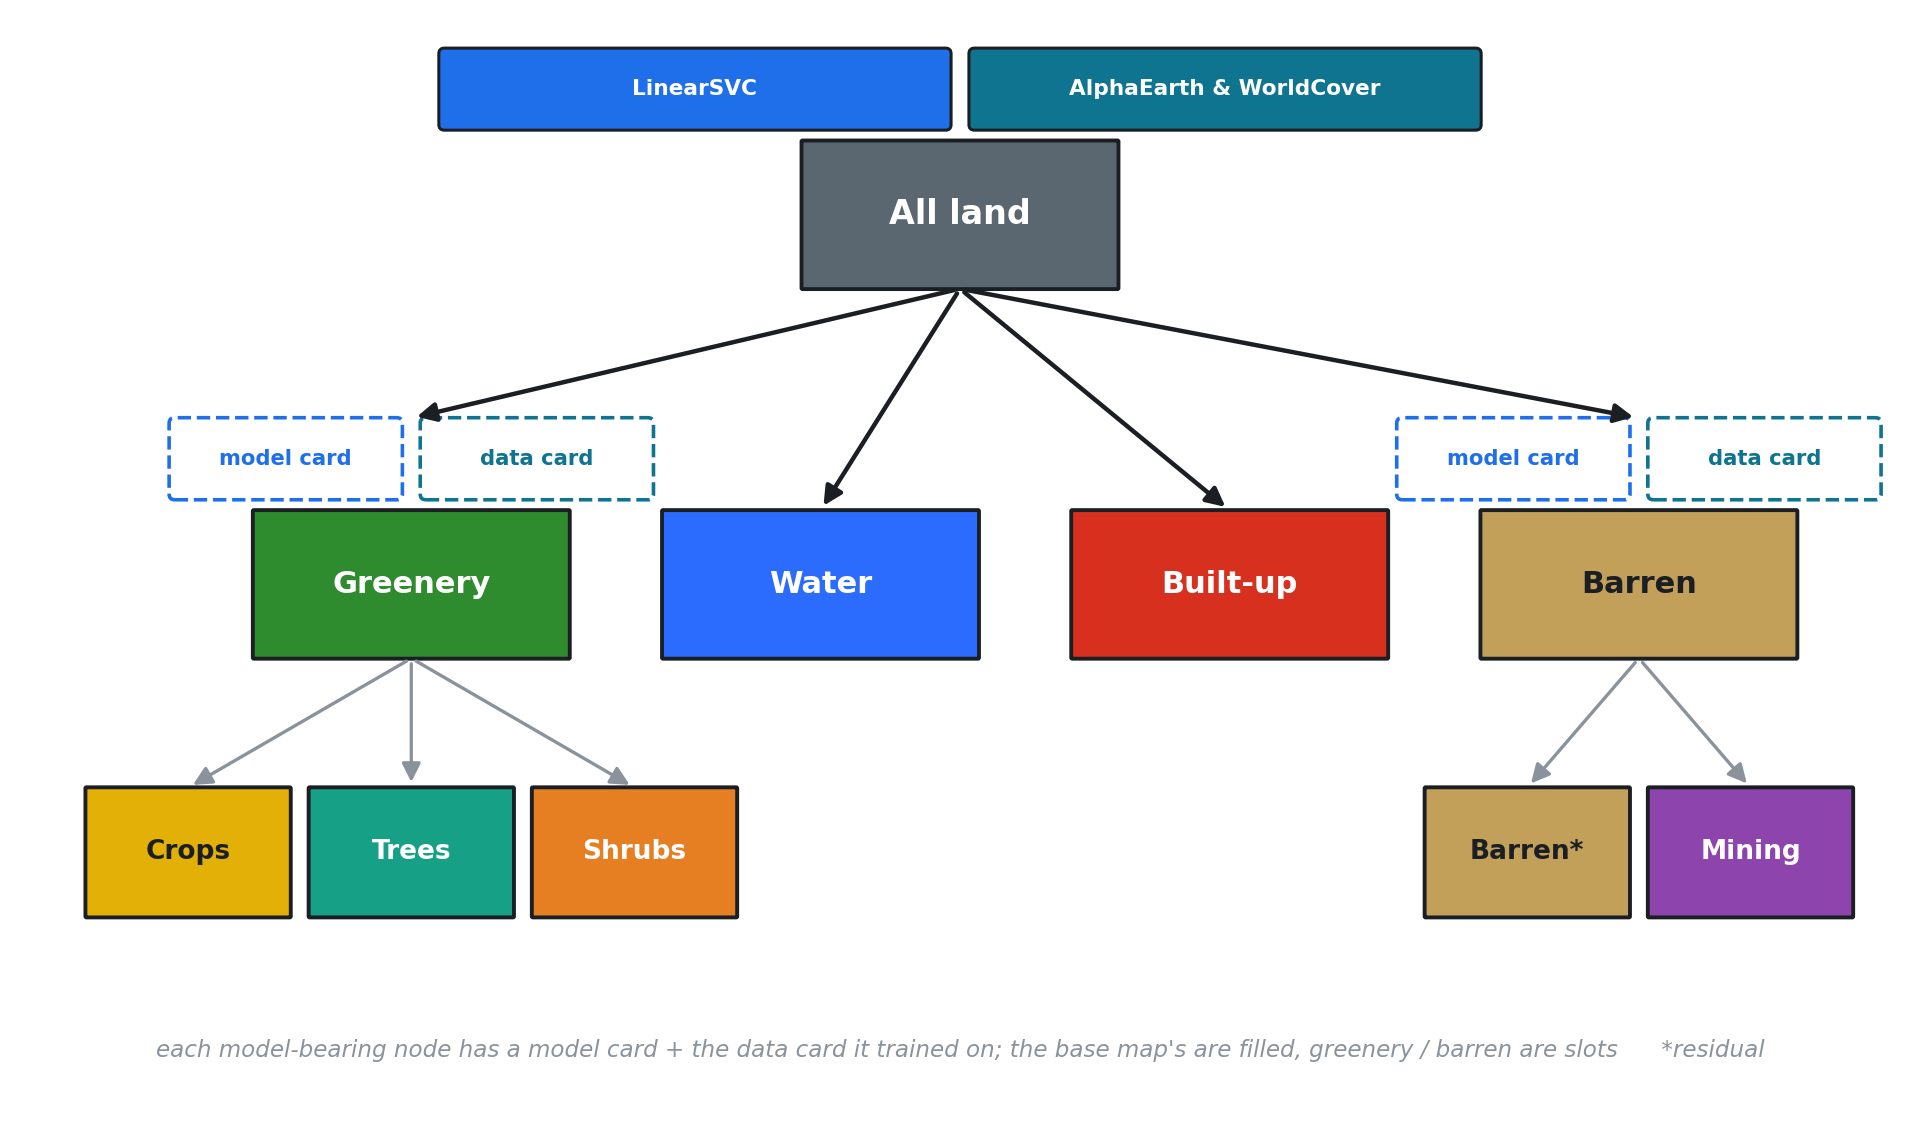
\includegraphics[width=0.96\linewidth]{figures/hierarchy_tree.png}\\[4pt]
{\footnotesize Each model-bearing node carries a \textbf{model card} + the \textbf{data card}
it trained on. The base map's are filled (LinearSVC; AlphaEarth + WorldCover); greenery /
barren are slots you fill. You can split or add at any level, including a \textbf{new base
class} under All land (which retrains the base map).}
\end{frame}

% ------------------------------------------------------------------
\begin{frame}{Our own taxonomy, growable at any level}
\begin{itemize}
  \item Start from 4 base classes, but the tree grows at \textbf{any} level: split a class,
  add a class, or even \textbf{add a new base class} (which retrains the base map).
  \item New classes usually map \textbf{into} our taxonomy where they fit (a seasonal /
  perennial water-body under water), so models stay comparable; if something genuinely doesn't
  fit, it can become a new base class.
  \item Standard taxonomies (WorldCover / USDA / IUCN) aren't the backbone. They show
  up \emph{only at retraining time}, as an optional cross-reference a user can attach.
\end{itemize}
\vspace{0.3em}
\begin{center}\footnotesize
\emph{Optional cross-reference (attached at retrain time):}\\[3pt]
\begin{tabular}{@{}llll@{}}
\toprule
our class & under & WorldCover & USDA \\
\midrule
crops  & greenery & Cropland (40)  & Cropland \\
trees  & greenery & Tree cover (10)& Forest land \\
mining & barren   & Bare/sparse (60)\,* & Extractive \\
\bottomrule
\end{tabular}\\[2pt]
* WorldCover has no ``mining'', which is \emph{why} you add it locally and roll it up to barren.
\end{center}
\end{frame}

% ------------------------------------------------------------------
\begin{frame}{Anatomy of the two cards}
\centering
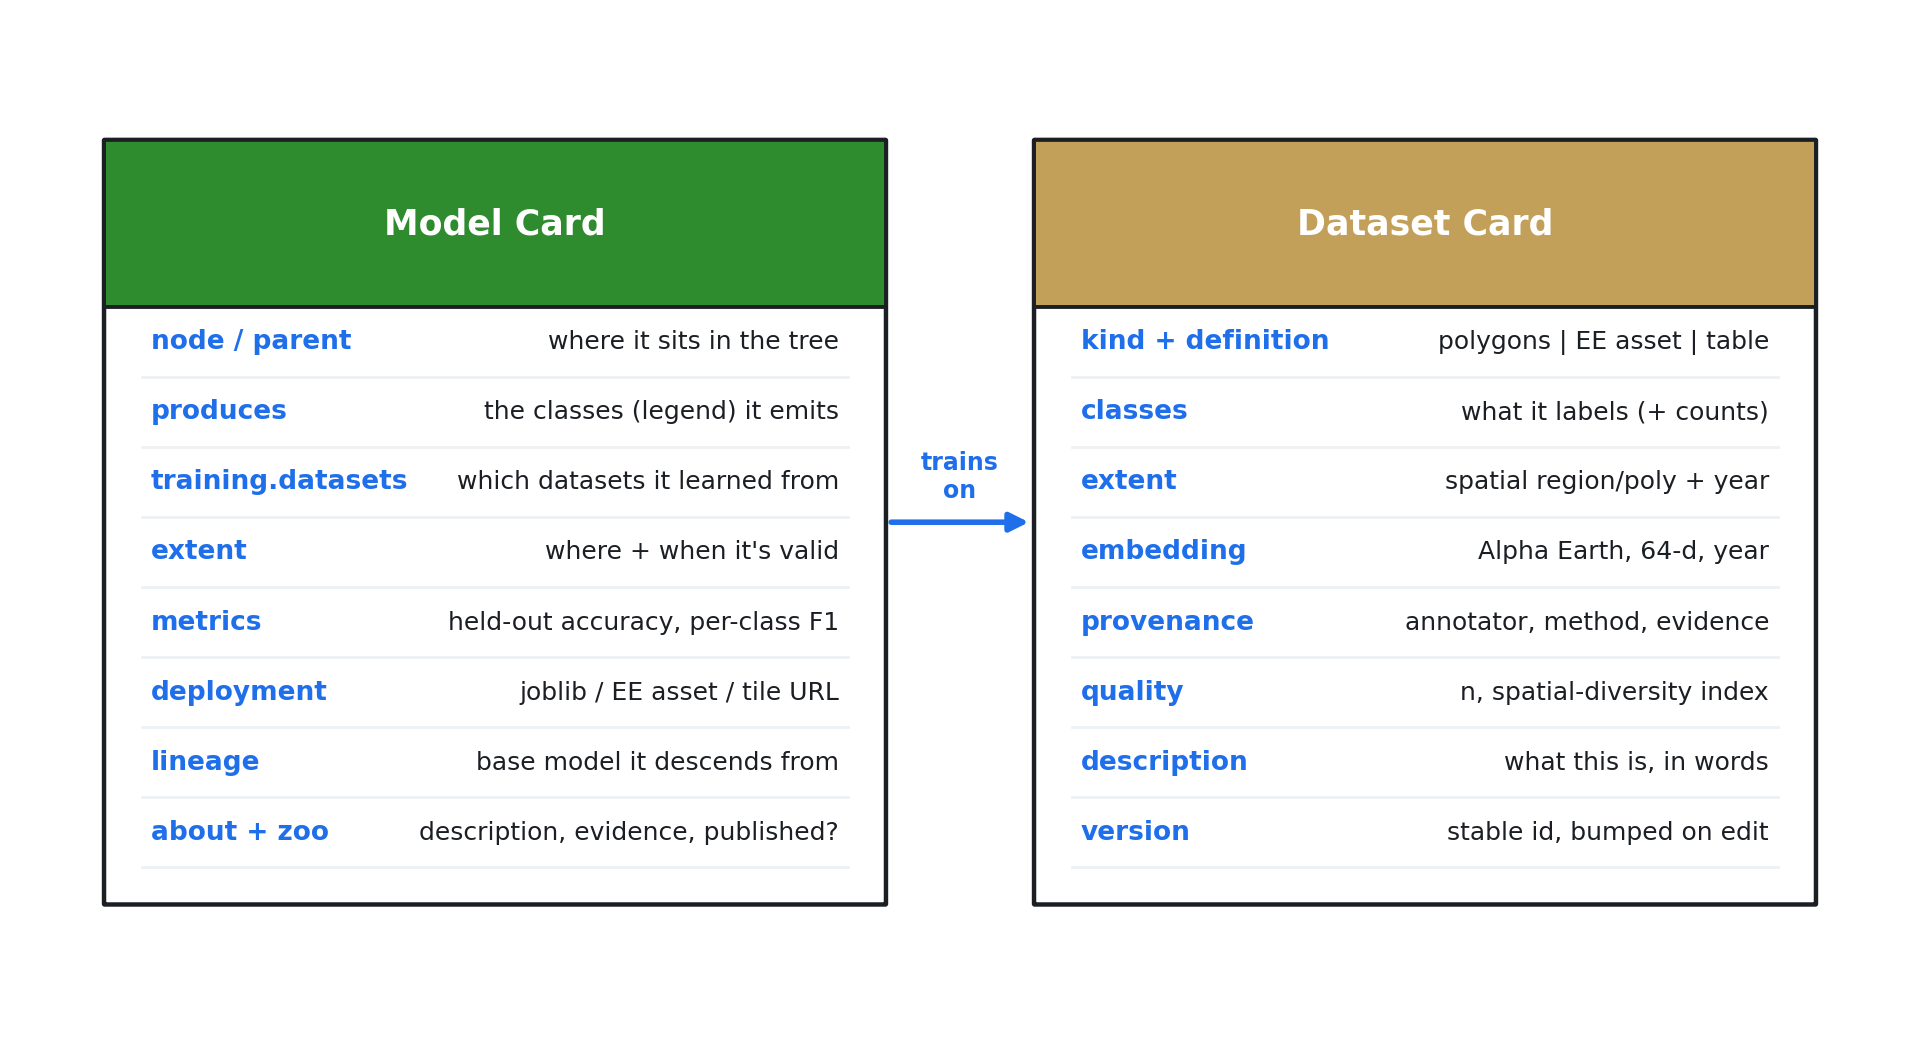
\includegraphics[width=0.95\linewidth]{figures/card_anatomy.png}\\[4pt]
{\footnotesize A model trains on one or more datasets; each card is a small JSON record (drafts next).}
\end{frame}

% ------------------------------------------------------------------
\begin{frame}[fragile]{Dataset Card: two ways to define a dataset}
\begin{lstlisting}[style=json]
{ "id": "ds_farmforest_crops_v1", "kind": "polygons",
  "description": "expert-delineated cropland parcels (crop positives)",  // describe it
  "classes": [ {"class":"crops","name":"Crops","count":110} ],
  "definition": {                      // (1) polygons  OR  (2) an EE asset
    "type": "polygons", "path": "data/examples/crops.geojson"
    // "type":"ee_asset","asset":"ESA/WorldCover/v200","band":"Map","code":20
  },
  "extent": { "spatial": {"type":"region","value":"India"}, "temporal": {"year":2024} },
  "provenance": { "annotator":"FarmForest expert", "method":"expert delineation",
                  "evidence":["drone imagery over IIT plots"] },   // how annotated + evidence
  "quality": { "n_polygons":110, "spatial_diversity":0.889 } }      // diversity / counts
\end{lstlisting}
\end{frame}

% ------------------------------------------------------------------
\begin{frame}[fragile]{Model Card: a classifier at one node}
\begin{lstlisting}[style=json]
{ "id": "mc_greenery_split_v1", "node": "greenery", "parent_class": "greenery",
  "topology": "per_node_split",
  "produces": [ {"class":"crops","std_mapping":{"worldcover":40}},
                {"class":"trees"}, {"class":"shrubs"} ],   // the legend it emits + map-out
  "training": { "datasets":["ds_farmforest_crops_v1","ds_farmforest_trees_v1",
                            "ds_worldcover_shrubs_v1"],
                "algo":"StandardScaler->LinearSVC",
                "balancing":{"method":"class_weight_balanced","residual_cap":8000} },
  "extent":  { "spatial":{"type":"region","value":"India"}, "temporal":{"year":2024} },
  "metrics": { "accuracy":0.963, "macro_f1":0.884, "eval":"polygon-holdout" },
  "deployment": { "ee_asset":null, "tile_url":null, "expressible_as_bandmath":true },
  "lineage":    { "base_model":"mc_base_pooled_v1", "derived_from":null },
  "about": { "description":"...", "intended_use":"...", "limitations":"shrubs weak" } }
\end{lstlisting}
\end{frame}

% ------------------------------------------------------------------
\begin{frame}[fragile]{The typed \texttt{extent} object (validity)}
One shape, three spatial forms plus a temporal field, so human AEZ labels and precise
geometries coexist. Used on \emph{both} cards.
\begin{lstlisting}[style=json]
"spatial": {"type":"region","value":"India"}      // world | AEZ-13 | district:...
//          {"type":"polygon","geojson":{...}}     // a drawn / uploaded boundary
//          {"type":"ee_asset","asset":"users/.../aez_13"}
"temporal": {"year":2024}                          // OR {"start":"2020","end":"2024"}
\end{lstlisting}
\begin{itemize}\footnotesize
  \item ``Is this area inside the model's extent?'' For a region, look up its geometry and
  test; for a polygon or EE asset, a direct geometry test.
  \item A dataset is valid \emph{somewhere}; a model is valid \emph{somewhere}; it's the same object.
  \item Space and time aren't the only axes: a model is also bound to the \textbf{embedding it
  was trained on} (Alpha Earth, with its version, year, and coverage). The object stays
  \emph{open} to such axes; we start with the ones we can actually check.
\end{itemize}
\end{frame}

% ------------------------------------------------------------------
\begin{frame}{Choosing the training data: the dataset panel}
\begin{columns}[T]
\begin{column}{0.54\textwidth}
\textbf{What the user picks from}
\begin{itemize}\small
  \item \textbf{Their own} polygons (drawn / uploaded).
  \item A \textbf{curated standard library} of pre-written cards for ESA WorldCover slices
  and USDA / IUCN refs. \emph{Offered, not web-searched} (provenance + reproducible).
  \item Tag each \textbf{positive} or \textbf{negative}; select / unselect freely.
\end{itemize}
\end{column}
\begin{column}{0.46\textwidth}
\textbf{Preferences applied to sampling}
\begin{itemize}\small
  \item \textbf{Spatial}: ``only my area of interest'' $\to$ clip to the AOI.
  \item \textbf{Temporal}: ``only year X'' $\to$ sets the sampling \& embedding year.
\end{itemize}
\vspace{0.3em}
{\footnotesize Recorded on the model as \texttt{training.datasets} + a \texttt{selection}
block (AOI + year) so a retrain is reproducible.}
\end{column}
\end{columns}
\end{frame}

% ------------------------------------------------------------------
\begin{frame}{Pick, refine, publish}
\centering
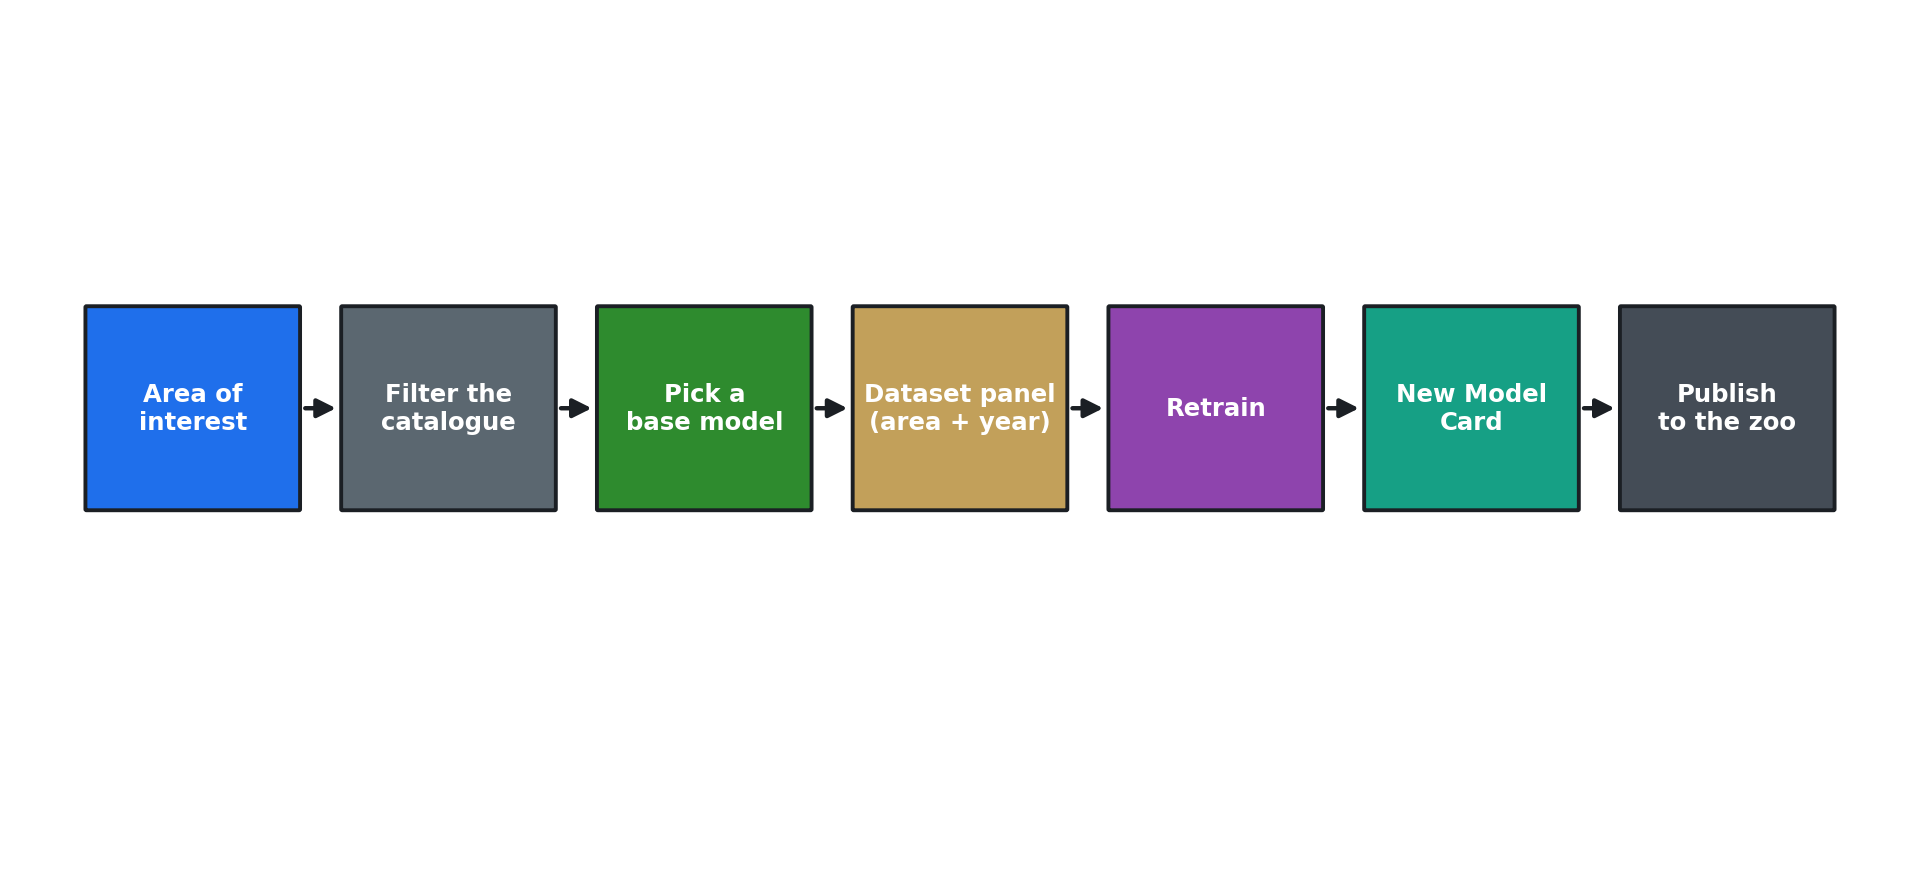
\includegraphics[width=0.97\linewidth]{figures/loop.png}
\end{frame}

% ------------------------------------------------------------------
\begin{frame}{Quality \& imbalance: guidelines baked in}
\begin{itemize}
  \item \textbf{Spatial diversity index} (dataset quality): Shannon entropy of sample
  locations over a coarse grid, normalized to $[0,1]$. $\approx 1$ = well spread; $\approx 0$
  = all from one spot. Flags ``100 polygons, all one district''. Measured on our demo data:
  crops \textbf{0.889}, mining \textbf{0.867}, trees \textbf{0.840} (healthily spread).
  \item \textbf{Imbalance guidelines} (before a split / add trains):
  \begin{itemize}\footnotesize
    \item compute the resulting class ratios; if skew passes a threshold (e.g.\ 5:1), warn;
    \item offer a fix: \emph{undersample} majority / \emph{oversample} minority / cap the
    residual (already capped at 8000) / re-weight;
    \item record the choice in \texttt{training.balancing}, and keep showing per-class metrics
    (a class can be present yet unlearnable, e.g.\ shrubs F1 0.695).
  \end{itemize}
\end{itemize}
{\footnotesize Ties to our finding: \emph{diversity}, not raw volume, moves accuracy on unseen regions.}
\end{frame}

% ------------------------------------------------------------------
\begin{frame}{Worked examples (real numbers, today's models)}
\begin{center}\footnotesize
\begin{tabular}{@{}lllr@{}}
\toprule
Model Card & node & topology & held-out acc. \\
\midrule
\texttt{mc\_base\_pooled\_v1}    & root     & base\_pooled    & 0.80 / 0.89$^\dagger$ \\
\texttt{mc\_greenery\_split\_v1} & greenery & per\_node\_split & 0.963 \\
\texttt{mc\_barren\_mining\_v1}  & barren   & per\_node\_split & 0.867 \\
\bottomrule
\end{tabular}\\[2pt]
$\dagger$ random India / balanced expert hold-out.
\end{center}
\begin{itemize}\footnotesize
  \item greenery: crops F1 0.965, trees 0.991, shrubs 0.695 (WorldCover-labelled, weak).
  \item mining (ADD = split + residual): mining F1 0.810 on 100 real polygons.
  \item Every field is filled from something we \textbf{already have}; for now the schema is
  \textbf{validated locally} against our existing models and datasets.
\end{itemize}
\end{frame}

% ------------------------------------------------------------------
\begin{frame}
\centering
\Large Thank you
\end{frame}

\end{document}
